\documentclass[12pt, twoside]{article}
\usepackage[letterpaper, margin=1in, headsep=0.5in]{geometry}
\usepackage[english]{babel}
\usepackage[utf8]{inputenc}
\usepackage{amsmath}
\usepackage{amsfonts}
\usepackage{amssymb}
\usepackage{tikz}
\usetikzlibrary{quotes, angles}
\usepackage{graphicx}
\usepackage{enumitem}
\usepackage{multicol}

\newif\ifmeta
\metatrue %print standards and topics tags

\title{Regents Geometry}
\author{Chris Huson}
\date{September 2020}

\usepackage{fancyhdr}
\pagestyle{fancy}
\fancyhf{}
\renewcommand{\headrulewidth}{0pt} % disable the underline of the header
\raggedbottom


\fancyhead[LE]{\thepage}
\fancyhead[RO]{\thepage \\ Name: \hspace{4cm} \,\\}
\fancyhead[LO]{BECA / Dr. Huson / Geometry 04 Analytic Geometry}

\begin{document}

\subsubsection*{4.15 Substitute packet: Angle situations}
\begin{enumerate}
\item In the diagram below $\angle AOB = x-35$ and $\displaystyle \angle COD = \frac{3}{4}(x+55)$. Find $\angle BOC$. \vspace{0.25cm}
\begin{flushright}
\begin{tikzpicture}[scale=1, rotate=0]
\draw [<->, thick] (0,0)--(155:5);
\draw [<->, thick] (-5,0)--(5,0);
\draw [->, thick] (0,0)--(0,4);
\draw (0,0)++(0.3,0)--++(0,0.3)--+(-0.3,0);
%\draw [fill] (-1,2.5) circle [radius=0.05] node[left ]{$B$};
\draw [fill] (155:3) circle [radius=0.05] node[below left]{$B$};
\draw [fill] (-4,0) circle [radius=0.05] node[below]{$A$}; 
\draw [fill] (0,0) circle [radius=0.05] node[below]{$O$};
\draw [fill] (0,3) circle [radius=0.05] node[left]{$C$};
\draw [fill] (4,0) circle [radius=0.05] node[below]{$D$};
\end{tikzpicture}
\end{flushright}

\item In the line segment $\overline{ABC}$, $\overline{AB}$ is twice as long as $\overline{BC}$. $AB=12x-6$ and $AC=15x+9$. Find $BC$.
\vspace{5cm}

\item In the diagram below $\angle AOB = 5x-15$ and $\angle DOE = 4x-4$. Find $m\angle AOB$. \vspace{0.25cm}
\begin{flushright}
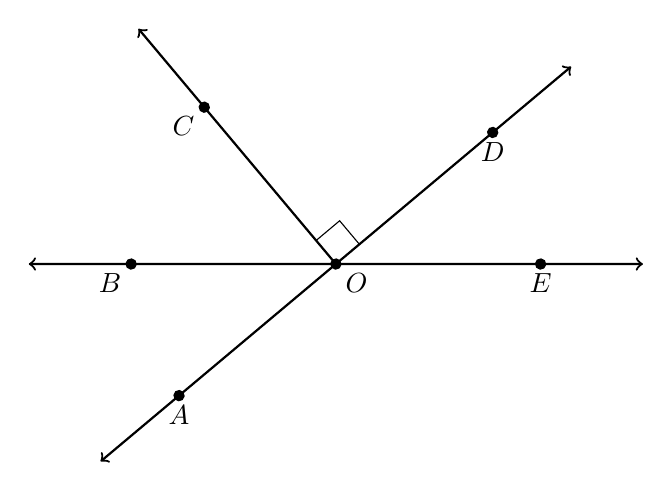
\begin{tikzpicture}[scale=1.3, rotate=40]
  \draw [<->, thick] (-40:3)--(0,0)--(140:3);
  \draw [<->, thick] (-3,0)--(3,0);
  \draw [->, thick] (0,0)--(0,3);
  \draw (0,0)++(0.3,0)--++(0,0.3)--+(-0.3,0);
  %\draw [fill] (-1,2.5) circle [radius=0.05] node[left ]{$B$};
  \draw [fill] (140:2) circle [radius=0.05] node[below left]{$B$};
  \draw [fill] (-2,0) circle [radius=0.05] node[below]{$A$}; 
  \draw [fill] (0,0) circle [radius=0.05] node[below right]{$O$};
  \draw [fill] (0,2) circle [radius=0.05] node[below left]{$C$};
  \draw [fill] (2,0) circle [radius=0.05] node[below]{$D$};
  \draw [fill] (-40:2) circle [radius=0.05] node[below]{$E$};
\end{tikzpicture}
\end{flushright}

\newpage
\item In the following two problems, solve for the value of $x$.
  \begin{multicols}{2}
    \begin{enumerate}
      \item   $\frac{4}{3}(6x-3)=x + 10$
      \item   $\frac{2}{5}(x-1)+\frac{5}{2}(1-x)=0$
    \end{enumerate}
  \end{multicols}
  \vspace{6cm}

\item Given the linear function $f(x)=-2x+14$.
\begin{multicols}{2}
  \begin{enumerate}
    \item Find $f(4)$
    \item   $f(x)=21$. Find $x$.
  \end{enumerate}
\end{multicols} \vspace{4cm}

\item Given two lines $\displaystyle f(x)=\frac{3}{2}x+8$ and $\displaystyle g(x)=-\frac{1}{4}x+5\frac{1}{2}$. Is the point $P(-2,5)$ on one line, both, or neither? \vspace{4cm} 


\end{enumerate}
\end{document}